% !TEX program = xelatex
\documentclass[12pt, a4paper]{ntut-report}
\usepackage[dvips,xetex]{graphicx}
\usepackage{ifpdf,mla}% <-- mla.sty requires ifpdf.sty, but (perversely) doesn't load it
%\usepackage{fontspec}
\usepackage{geometry}
\usepackage{lipsum}
\usepackage{xeCJK}
\usepackage{wallpaper}
\usepackage{pdfpages}
\usepackage{indentfirst}
\usepackage{setspace}
\usepackage{hyperref}
\usepackage{zhnumber}
\usepackage{titlesec}
\usepackage{amsmath}
\usepackage{mathspec}
\usepackage[backend=biber,sorting=none]{biblatex}
\usepackage{tabularx}
\usepackage{csquotes}
\usepackage{subcaption}
\usepackage{float}
\usepackage{placeins}
\usepackage{pgfplots}
\pgfplotsset{compat=1.18}

\MakeAutoQuote{“}{”}
\MakeOuterQuote{"}

\captionsetup{justification=centering,singlelinecheck=false,font={normalsize,stretch=2}}
\captionsetup[sub]{justification=centering,singlelinecheck=false,font={normalsize,stretch=2}}

\renewcommand{\baselinestretch}{1.5}
\xeCJKsetup{AutoFakeBold=true, AutoFakeSlant=true}
\setCJKmainfont{DFKai-SB.ttf} % 中文字體
\setmainfont{Times New Roman} % 英文字體
\setmathsfont(Digits,Latin){Times New Roman} % 數學模式之阿拉伯數字與拉丁字母統一使用 Times New Roman（符合 J1 規範 §3.4、§3.11）
\geometry{a4paper,total={297mm,210mm},top=4.5cm,bottom=0.75cm,left=2.5cm,right=2.5cm} % 頁面設定，不需修改
\pagestyle{plain} % 頁碼
\addbibresource{reference.bib}

%
% this file is encoded in utf-8
%

%% 這些設定值將會用於呈現在首頁上，請進行填入
%% Please fill in the information which will be shown on the cover and in the abstract. All Chinese and English information must be matched to each other. If you don’t have any Chinese information, please skip the Chinese ones, but all English Information is required.

%
% 中文論文設定值，請根據以下的範例進行填入
%

% 論文題目（中文）
% Thesis Title (Chinese)
\newcommand\cTitle{胸部 CT 影像於 COPD 輔助診斷之研究}

% 我的姓名（中文）
% My Name（Chinese）
\newcommand\myCname{張博翔}

% 指導教授的姓名 (中文)，使用頓號隔開 
% Advisor (Chinese), use “、” to separate names
\newcommand\advisorCname{劉建宏、尤信程}
% 共同指導教授的姓名 (中文)，使用頓號隔開
% Co-advisor (Chinese), use "、" to separate names
\newcommand\coAdvisorCname{}
% 校名 (中文)
% School Name（Chinese）
\newcommand\univCname{國立臺北科技大學}

% 系所名 (中文)
% Department Name（Chinese）
\newcommand\deptCname{資訊工程系碩士班}

% 學位名 (中文)
% Degree Name（Chinese）
\newcommand\degreeCname{碩士}

% 口試年份 (中文、民國)
% Year of Oral Defense（Chinese）
\newcommand\cYear{一百一十五}

% 口試月份 (中文)
% Month of Oral Defense（Chinese）
\newcommand\cMonth{七} 

% 畢業學年度 (中文)
% 如 112 學年度第2學期畢業，當時為民國113年6月，學年度即為112，不是113。
\newcommand\cAcademicYear{一百一十五}

% 畢業學期（中文）
% Academic Year (Chinese)
\newcommand\cGraduateSemester{二}

%
% 英文論文設定值，請根據以下的範例進行填入
%

% 論文題目 (英文）
% Thesis Title (Engslih)
\newcommand\eTitle{A Study on the Auxiliary Diagnosis of COPD using Chest CT images}

% 我的姓名（英文）
% My Name（English）
\newcommand\myEname{Chang, Po-Hsiang}

% 指導教授的姓名 (英文)，使用逗號隔開
% 例如：Dr. Kuo Jong-Yi, Dr. A B-C, ...
%
% Advisor (Ensligh), use “, ” to separate names
% e.g. Dr. Kuo Jong-Yi, Dr. A B-C, ...
\newcommand\advisorEname{Dr. Kuo Jong-Yi}
% 共同指導教授的姓名 (英文)，使用逗號隔開
% Co-advisor (English), use ", " to separate names
\newcommand\coAdvisorEname{}
% 校名（英文）
% School Name（English）
\newcommand\univEname{National Taipei University of Technology}

% 系所全名 (英文)
% Department Name（English）
\newcommand\fulldeptEname{Department of Computer Science and Information Engineering}

\newcommand\deptEname{Computer Science and Information Engineering}

% 學位名 (英文)
% Degree（English）
\newcommand\degreeEname{Master}

% 口試年份 (阿拉伯數字、西元)
% Year of Oral Defense（English）
\newcommand\eYear{2026}

% 口試月份 (英文)
% Month of Oral Defense（English）
\newcommand\eMonth{June}

%畢業級別；用於書背列印；若無此需要可忽略
\newcommand\GraduationClass{113}

%%%%%%%%%%%%%%%%%%%%%%
\setlength{\tocChNumberWidth}{2.4em}

\begin{document}

% 封面、不用浮水印 Cover without a watermark
\include{page/titlepage.tex}
% 留白頁、不用浮水印 Blank page without a watermark
\include{page/blankpage.tex}

% 新增浮水印 Add Watermarks
\CenterWallPaper{.64}{ntut-logo.png}

% 封面、要浮水印 Cover with a watermark
\input{page/titlepage.tex}
% 「學位論文口試委員會審定書」掃描檔，請檢附完整簽名之審定書掃描檔
% Please add "Oral Defense Committee Signature Form" with complete signatures.
\includepdf[pages=-]{static-page/signpage.pdf}

\pagenumbering{roman}

% 摘要頁（中文）Abstract (Chinese)
% If you don’t have Chinese abstract, please delete this one.
% 中文摘要頁
\begin{ZhAbstract}
    \begin{ZhAbstractItems}
        \noindent \text 關鍵詞：胸部 CT、COPD、量化生物標記、肺氣腫、自動化分類

    \end{ZhAbstractItems}

    \begin{ZhAbstractDescription}
        本研究提出一套以胸部 CT 影像為基礎之 COPD 輔助分析流程，從肺部分割、定量特徵擷取到分類模型訓練，建立可解釋之自動化判讀系統。系統以 54 筆臨床 CT 影像為資料來源，擷取 12 項具臨床意義之量化生物標記，包括全肺與分葉肺氣腫比例、血管與氣道相關指標、總肺容積及肺動脈直徑，並以五折交叉驗證訓練全連接神經網路進行 Normal/Abnormal 分類。實驗結果顯示，模型可達 92.59\% 之整體準確率與 0.9784 之 AUC；單一特徵分析亦顯示肺氣腫比例與肺容積對分類最具區辨能力。

        除量化生物標記外，本研究亦進一步將 3D CT 影像直接輸入深度模型，探討 COPD 相關肺功能表徵之預測與分級。實驗以 Mamba 與 Hybrid Mamba-Attention 架構為核心，分別進行肺功能塌陷角度回歸、角度三分類、排除中間灰區之極端二分類，以及 GOLD 嚴重度四分類。結果顯示，Hybrid Mamba-Attention 於角度回歸可達 15.85 度之 MAE 與 0.6699 之 Pearson 相關係數；在角度三分類與 GOLD 四分類中，結合資料增強與平衡取樣後，分別達到 0.5713 與 0.5323 之 Macro-F1，Balanced Accuracy 則為 0.6319 與 0.5222。於排除 132 至 151 度灰區後之極端二分類任務中，模型可達 0.8177 之 Macro-F1 與 0.8289 之 Balanced Accuracy，顯示合理的標籤設計與類別不平衡處理有助於提升小樣本 COPD CT 分類之可靠性。整體而言，胸部 CT 定量生物標記與 3D 深度影像模型可相互補足，作為 COPD 輔助診斷、肺功能表徵預測與疾病嚴重度評估之有效依據。
    \end{ZhAbstractDescription}
    
\end{ZhAbstract}

% 摘要頁（英文）Abstract (English)
% 英文摘要頁
\begin{EnAbstract}
    \begin{EnAbstractItems}
        \noindent \text Keyword: chest CT, COPD, quantitative biomarkers, Hybrid Mamba-Attention, TAP-CT, class imbalance

    \end{EnAbstractItems}

    \begin{EnAbstractDescription}
        Chronic obstructive pulmonary disease (COPD) is a chronic respiratory disease associated with airway obstruction and emphysema. Although pulmonary function testing remains the primary clinical basis for diagnosis, chest computed tomography (CT) provides structural information about lung parenchyma, airways, and vasculature, making it a potential source of auxiliary diagnostic evidence. This study develops a CT-based COPD auxiliary diagnostic framework that combines interpretable quantitative imaging biomarkers with 3D deep learning models, and evaluates its feasibility for Normal/Abnormal classification and pulmonary-function-related angle stratification.

        For quantitative analysis, 54 clinical chest CT scans were processed to generate lobe, vessel, and airway label maps. Twelve clinically meaningful biomarkers were extracted, including emphysema percentages, small vessel volume ratio, airway wall ratio, vessel density, airway-to-lung volume ratio, total lung volume, and pulmonary artery diameter. A fully connected neural network with stratified five-fold cross-validation achieved 92.59\% accuracy, an F1-score of 0.9355, and an AUC of 0.9784 for Normal/Abnormal classification, indicating that CT-derived biomarkers can provide interpretable evidence for COPD assessment.

        For 3D image-based learning, 66 CT scans with pulmonary-function-related labels were evaluated using Mamba, SwinUNETR, and Hybrid Mamba-Attention models. The tasks included Angle of Collapse (AC) three-class classification using $131^{\circ}$ and $152^{\circ}$ as thresholds, and binary classification after excluding cases between $132^{\circ}$ and $151^{\circ}$. With fused TAP-CT embeddings, AC three-class classification achieved 0.8209 accuracy, 0.6141 Macro-F1, and 0.6326 balanced accuracy, while binary classification achieved 0.9192 accuracy, 0.8763 Macro-F1, and 0.8778 balanced accuracy. Overall, CT-derived biomarkers and 3D models provide complementary evidence and may serve as references for COPD auxiliary diagnosis.
    \end{EnAbstractDescription}
    
\end{EnAbstract}

% 鳴謝 Acknowledgements
\begin{Thanks}

本論文得以完成，有賴多方師長與家人的支持與協助，謹致最誠摯之謝意。

首先感謝指導教授尤信程教授。在研究過程中，每當面臨方向不明、難以取捨之際，教授總能協助釐清優先次序，給予明確的研究建議；此外，教授積極促成本研究與醫療院所之合作，使資料蒐集得以順利進行，對本研究之推展貢獻甚鉅。

同時感謝指導教授劉建宏教授在研究態度上的提點。教授時常提醒應對自身工作保持嚴謹，即便外在要求不高，亦需自我維持一定水準，此觀念對本人之研究習慣有深遠影響。

此外，特別感謝振興醫院陳威廷醫師。陳醫師在百忙之中，慷慨提供胸部 CT 影像與肺功能檢查資料，並給予豐富的醫學背景知識、文獻建議與研究方向，使本研究得以在具臨床意義的問題框架下進行，對本論文之貢獻不可或缺。

最後，感謝家人長期以來的支持與包容，使本人得以專心完成學業。

\end{Thanks}
% 目錄、表目錄與圖目錄 Table of Contents, List of tables, List of figures
\include{page/table-of-content.tex}
 
\pagenumbering{arabic}

% 章節一 Chapter 1
\begin{ZhChapter}

\chapter{緒論}

\section{研究背景與動機}

慢性阻塞性肺病（Chronic Obstructive Pulmonary Disease, COPD）為一種與長期氣道阻塞、肺實質破壞及肺功能下降相關之慢性呼吸道疾病。臨床診斷主要依賴肺功能檢查，然而胸部電腦斷層影像（computed tomography, CT）能呈現肺實質、氣道與血管等結構變化，因此具有作為輔助診斷與疾病表徵分析之潛力。

\section{研究目的}

本研究旨在建立以胸部 CT 影像為基礎之 COPD 輔助診斷流程，並從可解釋量化特徵與三維影像模型兩個方向進行分析。前者擷取肺氣腫、氣道、血管與肺容積等量化生物標記，後者使用三維 CT 模型學習肺功能相關影像表徵。

\section{研究範圍與貢獻}

本研究範圍聚焦於胸部 CT 影像於 COPD 輔助診斷之應用，並不取代臨床肺功能檢查或醫師診斷。本研究所討論之分類與分級結果，主要作為影像輔助分析與研究性評估依據。主要貢獻如下：

\begin{enumerate}
    \item 建立胸部 CT 影像之 COPD 量化特徵分析流程，並以 12 項影像生物標記進行 Normal/Abnormal 分類。
    \item 評估三維 CT 深度學習模型於塌陷角角度分類與 GOLD 分級任務之可行性。
    \item 探討小樣本與類別不平衡情境下，資料增強與平衡取樣對模型效能之影響。
    \item 比較量化特徵方法與三維影像模型於 COPD 輔助診斷中之互補性。
\end{enumerate}

\section{論文架構}

本論文共分為五章。第二章整理相關背景與文獻，第三章說明研究材料與方法，第四章呈現實驗結果與討論，第五章總結研究成果、限制與未來方向。

\end{ZhChapter}

% 章節二 Chapter 2
\begin{ZhChapter}

\chapter{文獻回顧}

\section{慢性阻塞性肺病與肺功能檢查}
% TODO: COPD 臨床背景、病理特徵、肺功能檢查與 GOLD 分級。

\section{胸部 CT 於 COPD 評估之應用}
% TODO: CT 可觀察肺實質、氣道、血管等結構變化，作為肺功能外的輔助資訊。

\section{肺部、氣道與血管影像分割}
% TODO: 肺葉、氣道、血管分割方法，以及分割結果如何支援量化特徵。

\section{CT 量化生物標記}
% TODO: emphysema%、SVV%、vessel density、WA%、lung volume、PA diameter。

\section{三維醫學影像深度學習模型}
% TODO: 3D CNN、Transformer、SwinUNETR、Mamba、Hybrid Mamba-Attention。

\section{小樣本與類別不平衡問題}
% TODO: small sample、class imbalance、augmentation、balanced sampling、cross validation。

\section{評估指標}
% TODO: 分類與回歸指標，避免只看 accuracy。

\end{ZhChapter}

% 章節三 Chapter 3
\begin{ZhChapter}

\chapter{研究材料與方法}

\section{研究流程}

本研究以胸部電腦斷層影像為主要輸入，建立 COPD 輔助診斷與肺功能相關表徵預測流程。整體方法可分為兩條互補之分析分支：第一條分支為可解釋之 CT 量化生物標記分析，第二條分支為三維 CT 深度學習模型分析。前者將肺部、肺葉、血管與氣道等結構轉換為數值特徵，以評估 Normal/Abnormal 二元分類之可行性；後者直接以三維 CT volume 作為模型輸入，評估影像模型對肺功能相關塌陷角度分級與 GOLD 相關候選標籤之預測能力。

在 CT 量化生物標記分支中，原始 DICOM 影像先轉換為保留 Hounsfield unit 之 NIfTI volume，並依據適合肺部分析之胸部軸向影像序列建立後續輸入。轉換後之 CT 影像經肺部、肺葉、血管與氣道相關分割流程產生 label map，再依各結構遮罩計算肺氣腫比例、肺容積、血管密度、小血管體積比例、氣道相關比例與肺動脈直徑等特徵。由於此類特徵具有明確的解剖與病理對應關係，本研究將其視為可解釋影像生物標記，並以全連接神經網路進行 Normal/Abnormal 分類。

在三維 CT 深度學習分支中，轉換後之 NIfTI 影像不先壓縮為人工定義特徵，而是經尺寸統一、強度正規化與必要之資料增強後輸入三維模型。此分支包含 Mamba、SwinUNETR、Hybrid Mamba-Attention 與 TAP-CT 影像嵌入融合等模型設定，任務涵蓋 Normal/Abnormal 分類、連續塌陷角度迴歸、塌陷角度三分類、排除中間灰區後之極端二分類，以及 GOLD 相關候選分級分類。模型訓練與驗證皆以病人為單位切分資料，避免同一病人之原始影像與增強影像同時出現在訓練與驗證集合中。

兩條分支之目的並不完全相同。量化生物標記分支強調指標可解釋性與小樣本資料下的穩定分類能力；三維 CT 模型分支則強調由原始影像直接學習肺部空間表徵，補足人工定義特徵可能無法涵蓋的影像資訊。因此，本研究後續分別報告兩類方法之資料範圍、模型設定與評估結果，並於討論中比較其互補性與限制。

\section{資料集}

本研究資料由北投振興醫院合作醫師提供，包含病人胸部 CT 之 DICOM 影像及肺功能檢查（pulmonary function test, PFT）資料。原始 CT 影像以 DICOM series 形式儲存，經資料轉換流程產生 NIfTI volume 後，再依不同實驗目的建立量化特徵資料集與三維影像資料集。其他公開資料或外部資料僅作為前期工具測試、分割方法參考或未來擴充候選，未納入本研究已報告之主要模型訓練與評估。

量化生物標記分支使用其中 54 例胸部 CT，其中正常（Normal）21 例、異常或 COPD（Abnormal/COPD）33 例；其正常/異常二元標籤由合作醫師依 ATS/ERS 肺功能判讀標準與 PFT 結果判定\cite{stanojevic2022ersats}。此資料集用於肺部結構分割、量化參數擷取與正常/異常二元分類。由於本分支之核心目標為驗證 CT-derived biomarkers 是否能提供可解釋之 COPD 輔助判讀依據，因此每一例影像皆需具備可供後續特徵計算之 CT volume、肺部相關 label map 與量化參數輸出。另有後續新增之 12 例正常傾向 CT 已完成初步轉換，但未併入此 54 例量化特徵主實驗，以避免在未重跑完整分割、特徵擷取與交叉驗證流程前改變已報告之資料範圍。

三維 CT 深度學習分支使用 66 例可與 PFT 資料對應之 CT 影像。PFT 資料用於整理塌陷角度與 GOLD 相關候選標籤，並作為 Mamba、SwinUNETR、Hybrid Mamba-Attention 與 TAP-CT 融合模型訓練與驗證時之監督訊號。塌陷角度（Angle of Collapse, AC）係由肺功能檢查之呼氣流量容積曲線萃取的幾何指標，並非 CT 影像中的解剖角度。參考 Topalovic 等人提出之 AC 與肺氣腫關係，本研究採用 $131^{\circ}$ 與 $152^{\circ}$ 作為角度分級門檻\cite{topalovic2013anglecollapse}。

\begin{table}[htbp]
\centering
\caption{本研究影像資料組成}
\small
\begin{tabularx}{\textwidth}{l c X}
\hline
資料集 & 例數 & 標籤與實驗用途 \\
\hline
量化生物標記資料集 & 54 & 正常 21 例、異常或 COPD 33 例，標籤由醫師依 ATS/ERS 標準與 PFT 判定；用於肺部結構分割、量化參數擷取與正常/異常二元分類。\\
三維 CT 影像資料集 & 66 & 具由 PFT 整理之 AC 與 GOLD 相關候選標籤；用於三維 CT 模型訓練、塌陷角度分級、極端二分類與 GOLD 相關分類。\\
\hline
\end{tabularx}
\end{table}

AC 三分類任務將影像分為三類：$AC \leq 131^{\circ}$ 為 emphysema/abnormal-like 類別，$132^{\circ} \leq AC \leq 151^{\circ}$ 為 intermediate 類別，$AC \geq 152^{\circ}$ 為 normal-like 類別。原始 66 例資料中，三類樣本數分別為 14、5 與 47 例。由於 intermediate 類別樣本數較少且可能代表肺功能曲線表徵之灰區，本研究另設計 AC 極端二分類任務，排除 $132^{\circ}$ 至 $151^{\circ}$ 之 5 例，只保留 $AC \leq 131^{\circ}$ 與 $AC \geq 152^{\circ}$ 兩端較明確之 61 例資料。

GOLD 相關候選標籤則依肺功能檢查中 FEV1 佔預測值百分比進行整理，分為 GOLD 1、GOLD 2、GOLD 3 與 GOLD 4。於 66 例三維影像資料中，四類樣本數分別為 36、11、13 與 6 例。需要注意的是，此分組主要反映 FEV1 predicted 所對應之氣流受限嚴重度候選標籤；正式 COPD 診斷與 GOLD 分級仍需結合支氣管擴張劑後 FEV1/FVC、症狀、病史與臨床判讀。因此，本研究在方法與結果中將其稱為 GOLD 相關候選分級或肺功能導向分級，不將其直接等同於完整臨床診斷。

\begin{table}[htbp]
\centering
\caption{肺功能相關標籤定義}
\small
\begin{tabularx}{\textwidth}{l c c X}
\hline
標籤類型 & 類別條件 & 例數 & 說明 \\
\hline
AC 三分類 & $\leq 131^{\circ}$ & 14 & 肺氣腫或異常傾向 \\
AC 三分類 & $132^{\circ}$--$151^{\circ}$ & 5 & 中間灰區，於極端二分類中排除 \\
AC 三分類 & $\geq 152^{\circ}$ & 47 & 正常傾向 \\
AC 極端二分類 & 兩端類別 & 61 & 僅保留 $\leq 131^{\circ}$ 與 $\geq 152^{\circ}$ 樣本 \\
GOLD 相關候選分級 & GOLD 1--4 & 36、11、13、6 & 依 FEV1 預測值百分比整理 \\
\hline
\end{tabularx}
\end{table}

\section{資料前處理}
% TODO: DICOM to NIfTI、HU、resize/resampling、normalization。

\section{肺部結構分割與量化參數擷取}
% TODO: segmentation label、emphysema%、WA%、SVV%、vessel density、lung volume、PA diameter。

\section{量化生物標記分類模型}
% TODO: 12 features、standardization、MLP/FCNN、5-fold Normal/Abnormal classification。

\section{三維 CT 深度學習模型}
% TODO: 3D CT input、Mamba、SwinUNETR、Hybrid Mamba-Attention、tasks。

\section{TAP-CT 影像嵌入與融合策略}
% TODO: TAP-CT embedding、late fusion、attention fusion、ABMIL variants。

\section{交叉驗證、資料增強與平衡取樣}
% TODO: patient-level split、training-fold-only augmentation、balanced sampling。

\section{評估方法}
% TODO: classification metrics、regression metrics、macro/balanced metrics。

\end{ZhChapter}

% 章節四 Chapter 4
\begin{ZhChapter}

\chapter{實驗結果與討論}

\section{研究問題}

本章依研究流程彙整五項研究問題（Research Questions, RQs），分別評估 CT 量化特徵、三維影像模型與肺功能衍生標籤於 COPD 輔助判讀之表現。結果分析著重於模型效能、類別辨識均衡性及其臨床判讀意義。

\begin{list}{}{\setlength{\leftmargin}{4.2em}\setlength{\labelwidth}{3.4em}\setlength{\labelsep}{0.8em}\setlength{\itemsep}{0.35em}}
    \item[\textbf{RQ1：}]胸部 CT 影像擷取之量化生物標記，能否區分 COPD 正常與異常？
    \item[\textbf{RQ2：}]輸入三維 CT 之影像模型，是否能進行正常與異常分類？
    \item[\textbf{RQ3：}]三維 CT 影像模型是否能預測肺功能塌陷角度？
    \item[\textbf{RQ4：}]塌陷角度衍生之二分類與三分類標籤，是否有助於肺功能相關影像判讀？
    \item[\textbf{RQ5：}]三維 CT 影像模型能否辨識 GOLD 相關候選分級？
\end{list}

\section{實驗環境設定}

本研究實驗於本機工作站完成，硬體設備如表~\ref{tab:experiment_hardware} 所示。CT 量化生物標記分支於 Windows 環境執行，三維 CT 深度學習、塌陷角預測、GOLD 相關候選分級與 TAP-CT 相關實驗則於 Ubuntu 環境執行。兩分支之軟體環境整理如表~\ref{tab:quant_software} 與表~\ref{tab:deep_software}。

\begin{table}[htbp]
\centering
\caption{實驗硬體設備}
\label{tab:experiment_hardware}
\begingroup
\renewcommand{\arraystretch}{1.6}
\begin{tabularx}{0.95\textwidth}{|>{\centering\arraybackslash}p{0.28\textwidth}|>{\centering\arraybackslash}X|}
\hline
\textbf{項目} & \textbf{規格} \\
\hline
CPU & Intel Core i7-12700K 3.60GHz 12-Core Processor \\
\hline
GPU & NVIDIA GeForce RTX 4070 Ti SUPER \\
\hline
RAM & 32GB DDR4-3200MHz \\
\hline
Storage & 1TB NVMe SSD + 2TB SATA HDD \\
\hline
\end{tabularx}
\endgroup
\end{table}

\begin{table}[htbp]
\centering
\caption{CT 量化生物標記分支實驗環境}
\label{tab:quant_software}
\begingroup
\renewcommand{\arraystretch}{1.45}
\begin{tabularx}{0.95\textwidth}{|>{\centering\arraybackslash}p{0.28\textwidth}|>{\raggedright\arraybackslash}X|}
\hline
\textbf{項目} & \textbf{內容} \\
\hline
作業系統 & Windows 11 Pro 64-bit \\
\hline
分割與影像處理工具 & 3D Slicer、MONAI Auto3DSeg、AeroPath、SimpleITK \\
\hline
模型訓練與資料處理套件 & PyTorch、scikit-learn、NumPy、pandas \\
\hline
\end{tabularx}
\endgroup
\end{table}

\begin{table}[htbp]
\centering
\caption{三維 CT 深度學習分支實驗環境}
\label{tab:deep_software}
\begingroup
\renewcommand{\arraystretch}{1.45}
\begin{tabularx}{0.95\textwidth}{|>{\centering\arraybackslash}p{0.28\textwidth}|>{\raggedright\arraybackslash}X|}
\hline
\textbf{項目} & \textbf{內容} \\
\hline
作業系統 & Ubuntu 24.04.4 LTS (Noble Numbat)，Linux kernel 6.17.0-29-generic，x86\_64 \\
\hline
深度學習環境 & Python 3.11、PyTorch 2.8.0、CUDA 12.8、MONAI \\
\hline
醫學影像與資料處理套件 & SimpleITK、nibabel、scikit-learn、pandas、matplotlib \\
\hline
TAP-CT 相關套件 & transformers、timm、einops \\
\hline
\end{tabularx}
\endgroup
\end{table}

\section{實驗結果分析}
\subsection{RQ1 量化特徵二分類結果}

RQ1 以 12 項 CT 衍生量化生物標記作為輸入，採五折交叉驗證評估 Normal 與 Abnormal 個案之辨識能力，結果如表~\ref{tab:rq1_quant_result} 與圖~\ref{fig:rq1_quant_cm} 所示。整體 Accuracy 為 0.9259，AUC 為 0.9784，顯示量化特徵已能有效區分兩類個案。Precision 與 Specificity 皆為 1.0000，代表本實驗未將 Normal 個案誤判為 Abnormal；Sensitivity 為 0.8788，仍有 4 筆 Abnormal 個案被判為 Normal。此結果說明肺氣腫比例、肺容積、血管與氣道等特徵具有輔助判讀價值，但異常個案漏判仍是後續模型優化的主要問題。

\begin{table}[htbp]
\centering
\caption{RQ1 量化特徵二分類結果}
\label{tab:rq1_quant_result}
\begingroup
\renewcommand{\arraystretch}{1.25}
\begin{tabularx}{0.75\textwidth}{>{\raggedright\arraybackslash}X >{\centering\arraybackslash}X >{\centering\arraybackslash}X}
\hline
指標 & 整體結果 & 五折平均 \\
\hline
Accuracy & 0.9259 & \(0.9273 \pm 0.0680\) \\
Precision & 1.0000 & \(1.0000 \pm 0.0000\) \\
Sensitivity & 0.8788 & \(0.8810 \pm 0.1086\) \\
Specificity & 1.0000 & -- \\
F1-score & 0.9355 & \(0.9331 \pm 0.0626\) \\
AUC & 0.9784 & \(0.9657 \pm 0.0430\) \\
\hline
\end{tabularx}
\endgroup
\end{table}

\begin{figure}[htbp]
\centering
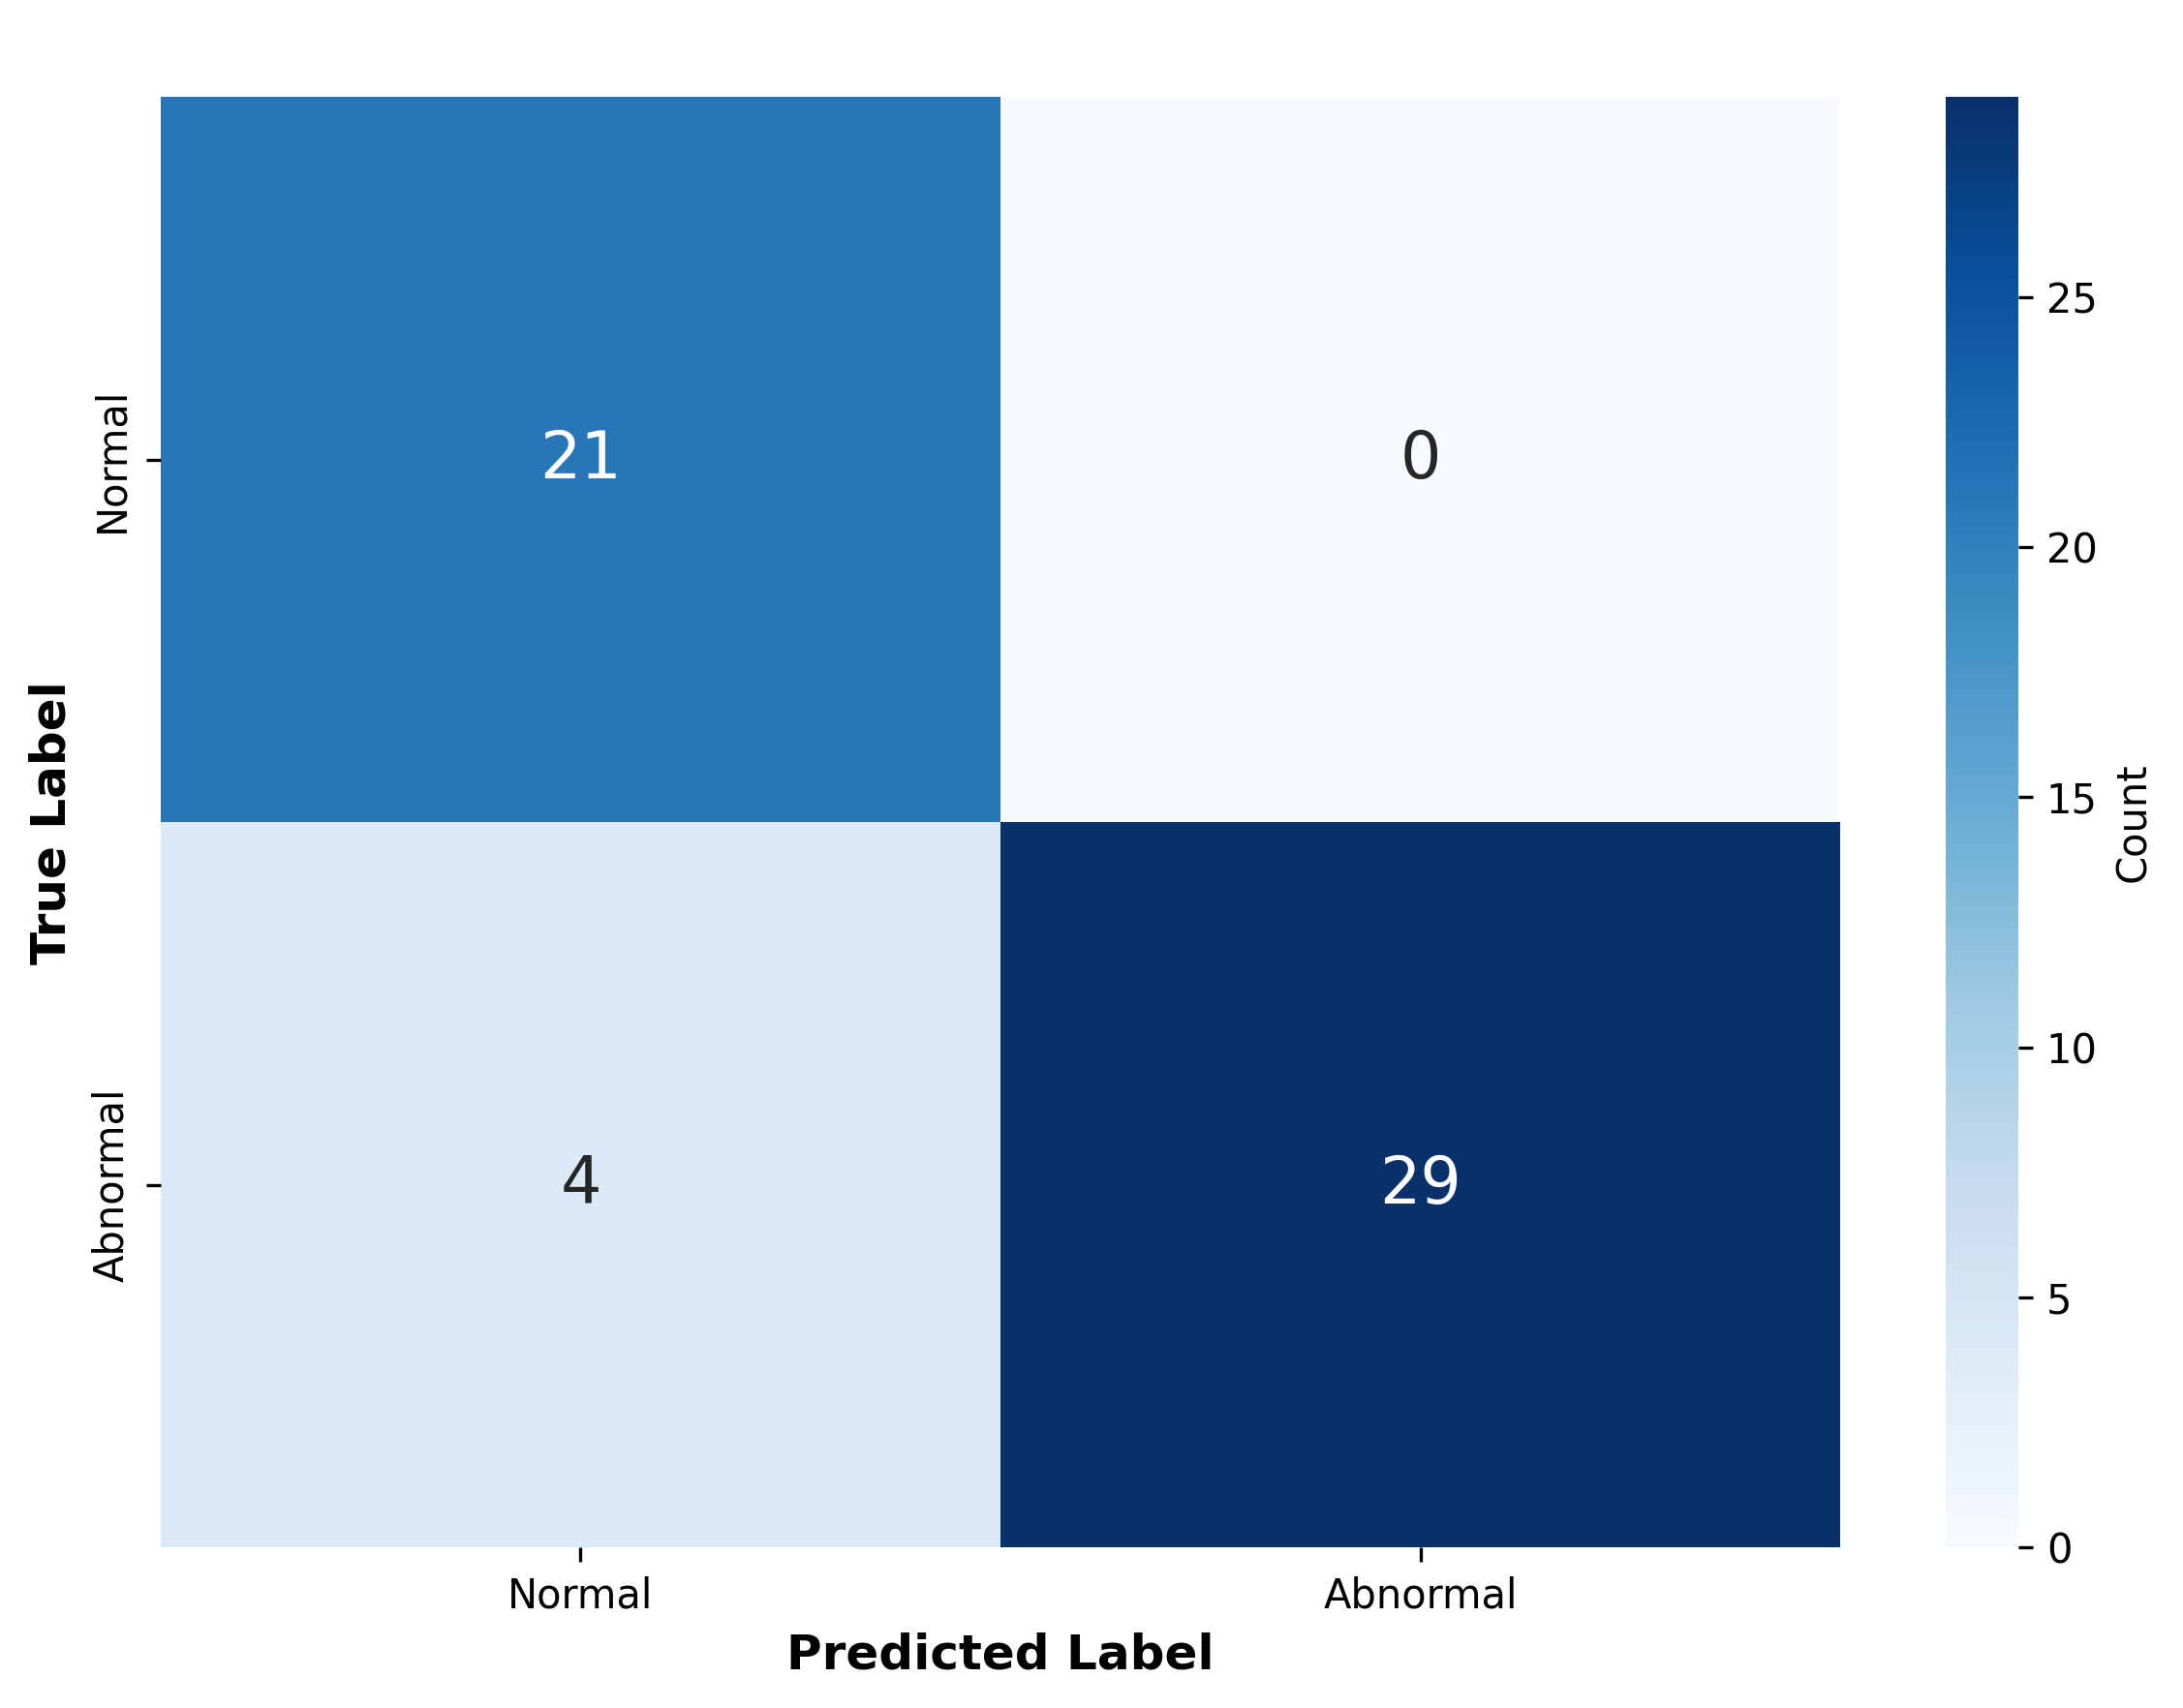
\includegraphics[width=0.80\textwidth]{figures/kfold_confusion_matrix.png}
\caption{RQ1 量化特徵二分類混淆矩陣圖}
\label{fig:rq1_quant_cm}
\end{figure}
\FloatBarrier

\subsection{RQ2 三維影像模型二分類結果}

RQ2 評估三維 CT 影像模型於 Normal/Abnormal 分類之表現。本研究採用五折平均 AUC 最高之 nnMamba e5 設定作為代表結果，各指標均以平均值與標準差呈現，如表~\ref{tab:rq2_3d_binary} 所示。

\begin{table}[htbp]
\centering
\caption{RQ2 最佳三維影像二分類結果}
\label{tab:rq2_3d_binary}
\begingroup
\renewcommand{\arraystretch}{1.25}
\begin{tabular}{l c}
\hline
指標 & 五折平均結果 \\
\hline
AUC & \(1.0000 \pm 0.0000\) \\
Accuracy & \(0.9409 \pm 0.0422\) \\
Sensitivity & \(0.9019 \pm 0.0718\) \\
Specificity & \(1.0000 \pm 0.0000\) \\
\hline
\end{tabular}
\endgroup
\end{table}

最佳三維影像模型之 AUC 為 \(1.0000 \pm 0.0000\)，Accuracy 為 \(0.9409 \pm 0.0422\)，Specificity 亦達 \(1.0000 \pm 0.0000\)。Sensitivity 為 \(0.9019 \pm 0.0718\)，顯示模型仍可能漏判部分異常個案。與 RQ1 相比，三維影像模型可直接學習三維 CT 體積資料之空間表徵，整體 Accuracy 與 AUC 略高；但其臨床應用仍需處理異常個案漏判及模型可解釋性不足的問題。
\FloatBarrier

\subsection{RQ3 三維影像角度預測結果}

RQ3 評估三維影像模型預測塌陷角連續值之能力，結果如表~\ref{tab:rq3_ac_regression} 所示。

\begin{table}[htbp]
\centering
\caption{RQ3 塌陷角連續值迴歸結果}
\label{tab:rq3_ac_regression}
\begingroup
\small
\renewcommand{\arraystretch}{1.25}
\begin{tabularx}{\textwidth}{>{\raggedright\arraybackslash}X c c c c}
\hline
模型 & MAE & RMSE & \(R^2\) & Pearson \\
\hline
Hybrid Mamba-Attention & \(15.8512 \pm 4.7756\) & 21.2647 & 0.1723 & 0.6699 \\
Mamba & \(17.1180 \pm 2.5754\) & 23.9086 & 0.0314 & 0.3413 \\
SwinUNETR & \(19.0884 \pm 2.8357\) & 24.3769 & -0.0012 & 0.1898 \\
\hline
\end{tabularx}
\endgroup
\end{table}

\begin{figure}[H]
\centering
\begin{tikzpicture}
\begin{axis}[
    ybar,
    width=0.95\textwidth,
    height=6cm,
    ymin=0,
    ymax=22,
    ylabel={MAE},
    symbolic x coords={Hybrid,Mamba,SwinUNETR},
    xtick=data,
    bar width=18pt,
    enlarge x limits=0.15,
    nodes near coords,
    nodes near coords style={font=\small, /pgf/number format/fixed, /pgf/number format/precision=2},
    ymajorgrids=true,
    grid style={gray!25}
]
\addplot coordinates {(Hybrid,15.8512) (Mamba,17.1180) (SwinUNETR,19.0884)};
\end{axis}
\end{tikzpicture}
\caption{塌陷角連續值迴歸平均絕對誤差比較}
\label{fig:rq3_ac_regression}
\end{figure}

Hybrid Mamba-Attention 取得最低 MAE，平均誤差為 \(15.8512 \pm 4.7756\)，Pearson correlation 為 0.6699，皆優於其他模型。Mamba 與 SwinUNETR 之 MAE 分別為 \(17.1180 \pm 2.5754\) 與 \(19.0884 \pm 2.8357\)。結果顯示，在 Mamba 表徵後加入 attention bridge，可補充塌陷角預測所需之影像資訊；然而 \(R^2\) 仍偏低，表示單以 CT 影像精準估計連續肺功能指標仍具限制。
\FloatBarrier

\subsection{RQ4 塌陷角衍生分類結果}

RQ4 比較塌陷角衍生標籤於二分類與三分類任務中的可辨識性。以下先呈現排除 \(132^{\circ}\)--\(151^{\circ}\) 中間灰區後之 AC 二分類，再呈現保留 intermediate 類別之 AC 三分類。\texttt{baseline} 代表未加入 TAP-CT 融合或虛擬補強之原始三維 CT 設定；\texttt{pooled} 代表使用凍結之 TAP-CT 掃描嵌入，並以 ABMIL 分類頭彙整為病人層級表徵；\texttt{aug100} 與 \texttt{aug300} 則代表每類虛擬補強至 100 或 300 筆。

AC 二分類結果如表~\ref{tab:rq4_ac_binary} 所示。

\begin{table}[htbp]
\centering
\caption{RQ4 AC 二分類結果}
\label{tab:rq4_ac_binary}
\begingroup
\footnotesize
\renewcommand{\arraystretch}{1.25}
\setlength{\tabcolsep}{3pt}
\begin{tabular}{p{0.30\textwidth} p{0.14\textwidth} c c c}
\hline
模型 & 設定 & Accuracy & Macro-F1 & Bal. acc. \\
\hline
TAP-CT late fusion & aug100 & \(0.9192 \pm 0.0718\) & \(0.8763 \pm 0.1186\) & \(0.8778 \pm 0.1333\) \\
Hybrid Mamba-Attention & aug100 & \(0.8692 \pm 0.0656\) & \(0.8177 \pm 0.0761\) & \(0.8289 \pm 0.0963\) \\
Hybrid Mamba-Attention & baseline & \(0.7705 \pm 0.0323\) & \(0.4350 \pm 0.0101\) & \(0.5000 \pm 0.0000\) \\
\hline
\end{tabular}
\endgroup
\end{table}

排除中間灰區後，AC 二分類表現明顯提升。TAP-CT late fusion 搭配 aug100 取得最高 Accuracy（\(0.9192 \pm 0.0718\)）與 Macro-F1（\(0.8763 \pm 0.1186\)），相較 Hybrid Mamba-Attention baseline 之 Macro-F1 0.4350 有大幅改善。此結果指出，低角度異常傾向與高角度正常傾向兩端樣本具有較明確的影像差異。

AC 三分類結果如表~\ref{tab:rq4_ac_3class} 所示。

\begin{table}[htbp]
\centering
\caption{RQ4 AC 三分類結果}
\label{tab:rq4_ac_3class}
\begingroup
\footnotesize
\renewcommand{\arraystretch}{1.25}
\setlength{\tabcolsep}{3pt}
\begin{tabular}{p{0.30\textwidth} p{0.14\textwidth} c c c}
\hline
模型 & 設定 & Accuracy & Macro-F1 & Bal. acc. \\
\hline
TAP-CT late fusion & aug100 & \(0.8209 \pm 0.0939\) & \(0.6141 \pm 0.1403\) & \(0.6326 \pm 0.1803\) \\
TAP-CT-S-2.5D late fusion & aug100 & \(0.8352 \pm 0.0831\) & \(0.5884 \pm 0.0756\) & \(0.5933 \pm 0.0952\) \\
TAP-CT ABMIL S-3D & pooled & \(0.7132 \pm 0.0846\) & \(0.5883 \pm 0.1381\) & \(0.6400 \pm 0.2036\) \\
Hybrid Mamba-Attention & baseline & \(0.7879 \pm 0.1018\) & \(0.5861 \pm 0.1546\) & \(0.6200 \pm 0.1154\) \\
Hybrid Mamba-Attention & aug300 & \(0.7593 \pm 0.1173\) & \(0.5713 \pm 0.0748\) & \(0.6319 \pm 0.1160\) \\
\hline
\end{tabular}
\endgroup
\end{table}

AC 三分類中，TAP-CT late fusion 搭配 aug100 取得最高 Macro-F1（\(0.6141 \pm 0.1403\)），Accuracy 為 \(0.8209 \pm 0.0939\)。TAP-CT-S-2.5D late fusion 雖有最高 Accuracy（\(0.8352 \pm 0.0831\)），但 Macro-F1 較低，表示類別間辨識較不均衡。相較於二分類，三分類需額外辨識樣本數較少且界線較模糊的 intermediate 類別，因此 Macro-F1 明顯下降，顯示中間灰區會增加肺功能相關影像判讀難度。

\begin{figure}[htbp]
\centering
\begin{tikzpicture}
\begin{axis}[
    ybar,
    width=0.95\textwidth,
    height=6.2cm,
    ymin=0,
    ymax=0.95,
    ylabel={Score},
    symbolic x coords={Late fusion,TAP-CT-S,ABMIL,Hybrid,Hybrid aug300},
    xtick=data,
    x tick label style={rotate=20, anchor=east},
    bar width=8pt,
    enlarge x limits=0.14,
    legend style={at={(0.5,-0.28)}, anchor=north, legend columns=2},
    ymajorgrids=true,
    grid style={gray!25}
]
\addplot coordinates {(Late fusion,0.8209) (TAP-CT-S,0.8352) (ABMIL,0.7132) (Hybrid,0.7879) (Hybrid aug300,0.7593)};
\addplot coordinates {(Late fusion,0.6141) (TAP-CT-S,0.5884) (ABMIL,0.5883) (Hybrid,0.5861) (Hybrid aug300,0.5713)};
\legend{Accuracy, Macro-F1}
\end{axis}
\end{tikzpicture}
\caption{塌陷角三分類效能比較}
\label{fig:rq4_ac_3class}
\end{figure}
\FloatBarrier

\subsection{RQ5 三維影像 GOLD 相關候選分級結果}

RQ5 評估三維影像模型對 GOLD 相關候選分級之辨識能力，結果如表~\ref{tab:rq5_gold_result} 所示。由於四類樣本數不均且 GOLD 4 樣本數最少，本研究以 Macro-F1 作為主要比較指標，以降低多數類別對 Accuracy 的影響。\texttt{aug36/class} 與 \texttt{aug200/class} 分別代表於各訓練折中將類別虛擬補強至每類 36 或 200 筆，並搭配平衡取樣訓練。

\begin{table}[htbp]
\centering
\caption{RQ5 GOLD 相關候選分級結果}
\label{tab:rq5_gold_result}
\begingroup
\footnotesize
\renewcommand{\arraystretch}{1.25}
\setlength{\tabcolsep}{3pt}
\begin{tabular}{p{0.25\textwidth} p{0.16\textwidth} c c c c}
\hline
模型 & 設定 & Folds & Accuracy & Macro-F1 & Bal. acc. \\
\hline
Hybrid Mamba-Attention & \shortstack[l]{aug36\\class} & 3 & \(0.5606 \pm 0.1134\) & \(0.5323 \pm 0.0479\) & \(0.5222 \pm 0.0463\) \\
Hybrid Mamba-Attention & \shortstack[l]{基準\\F1 較佳} & 3 & \(0.5152 \pm 0.1868\) & \(0.4639 \pm 0.1645\) & \(0.5194 \pm 0.0834\) \\
Hybrid Mamba-Attention & \shortstack[l]{aug200\\class} & 3 & \(0.5606 \pm 0.0773\) & \(0.4436 \pm 0.0674\) & \(0.4611 \pm 0.0307\) \\
Hybrid Mamba-Attention & \shortstack[l]{基準\\Accuracy 較佳} & 3 & \(0.5758 \pm 0.0857\) & \(0.4355 \pm 0.0532\) & \(0.5000 \pm 0.0780\) \\
SwinUNETR & baseline & 3 & \(0.4444 \pm 0.1361\) & \(0.3144 \pm 0.1559\) & \(0.3472 \pm 0.1084\) \\
Mamba & baseline & 3 & \(0.4259 \pm 0.1458\) & \(0.3107 \pm 0.0392\) & \(0.3674 \pm 0.0606\) \\
\hline
\end{tabular}
\endgroup
\end{table}

Hybrid Mamba-Attention 搭配 aug36/class 取得最高 Macro-F1（\(0.5323 \pm 0.0479\)），Accuracy 為 \(0.5606 \pm 0.1134\)，Balanced accuracy 為 \(0.5222 \pm 0.0463\)。三個 fold 的 Accuracy 分別為 0.6818、0.5909 與 0.4091，顯示小樣本四分類仍有明顯 fold 間變異。相較於 F1 較佳之基準設定，aug36/class 將 Macro-F1 由 0.4639 提升至 0.5323；Accuracy 較佳之基準設定雖有最高 Accuracy 0.5758，但 Macro-F1 僅 0.4355，代表整體正確率較高不必然反映各類別辨識能力。aug200/class 的 Accuracy 與 aug36/class 相同，但 Macro-F1 降至 0.4436，顯示過量補強未能改善類別平均表現。

\begin{figure}[htbp]
\centering
\begin{tikzpicture}
\begin{axis}[
    ybar,
    width=0.95\textwidth,
    height=6.2cm,
    ymin=0,
    ymax=0.7,
    ylabel={Score},
    symbolic x coords={Hybrid aug36,Base F1,Hybrid aug200,Base Acc,SwinUNETR,Mamba},
    xtick=data,
    x tick label style={rotate=24, anchor=east},
    bar width=8pt,
    enlarge x limits=0.14,
    legend style={at={(0.5,-0.28)}, anchor=north, legend columns=2},
    ymajorgrids=true,
    grid style={gray!25}
]
\addplot coordinates {(Hybrid aug36,0.5606) (Base F1,0.5152) (Hybrid aug200,0.5606) (Base Acc,0.5758) (SwinUNETR,0.4444) (Mamba,0.4259)};
\addplot coordinates {(Hybrid aug36,0.5323) (Base F1,0.4639) (Hybrid aug200,0.4436) (Base Acc,0.4355) (SwinUNETR,0.3144) (Mamba,0.3107)};
\legend{Accuracy, Macro-F1}
\end{axis}
\end{tikzpicture}
\caption{GOLD 候選分級分類效能比較}
\label{fig:rq5_gold_result}
\end{figure}

\end{ZhChapter}

% 章節五 Chapter 5
\begin{ZhChapter}

\chapter{結論與未來展望}

\section{研究結論}
% TODO: 總結量化特徵與 3D 模型的主要發現。

\section{研究貢獻}
% TODO: 呼應 1.3，不要重複太多。

\section{研究限制}
% TODO: sample size、heterogeneity、segmentation quality、label definition、external validation。

\section{未來工作}
% TODO: more data、external validation、better airway/vessel segmentation、clinical multimodal model。

\end{ZhChapter}

% 原始模板範例已保留於 chapter/example/，需要參考格式時再打開，不需 include。

% 參考文獻，請在段落上隨意註解，你同時需要 reference.bib
\chapter*{參考文獻}
\addcontentsline{toc}{chapter}{參考文獻}
\begingroup
\setlength{\emergencystretch}{2em}
\printbibliography[heading=none]
\endgroup


\end{document}
